\usetheme[height=0mm]{Rochester}
\usecolortheme{}
\usefonttheme[onlylarge]{structurebold}
\setbeamerfont*{frametitle}{size=\normalsize,series=\bfseries}
\setbeamertemplate{navigation symbols}{}
\setbeamercovered{dynamic}
\setbeamertemplate{itemize item}[triangle]
\setbeamertemplate{itemize subitem}[triangle]

%  use Darmstadt if commenting the next line
\usepackage[footheight=1em]{beamerthemeboxes}
\usepackage[natbib=true,backend=biber,citestyle=authoryear,maxbibnames=2]{biblatex}
\bibliography{../bib/biblio_julyan} % ../bib/stats,../bib/statsjulyan,../bib/learningjulyan

%\let\oldcite=\cite
%\renewcommand\cite[1]{\hyperlink{#1}{\textcolor{gray}{\oldcite{#1}}}}
%\let\oldcite=\citet
%\renewcommand\citet[1]{\hyperlink{#1}{\textcolor{gray}{\oldcite{#1}}}}
%\let\oldcitep=\citep
%\renewcommand\citep[1]{\hyperlink{#1}{\textcolor{gray}{\oldcitep{#1}}}}

\usepackage{amsmath,amssymb,amsthm,bbm}             % AMS Math
\usepackage[utf8]{inputenc}
\usepackage[english]{babel}
%\usepackage{myAlgorithm}
\usepackage{xcolor}
\usepackage{graphicx}
\usepackage{subfigure}
\usepackage{hyperref}
\usepackage{mathtools}
\usepackage{mathrsfs}
\usepackage{animate}
%\usepackage{fontawesome5} % twitter bird


\usepackage{color}
%\usepackage[citecolor=blue]{hyperref}
%\RequirePackage[citecolor=blue]{hyperref}
%\usepackage{animate}
\usepackage{xspace}
\usepackage{algorithm, algorithmic}
\usepackage{mathrsfs,dsfont}
\usepackage{amssymb,amsmath,amsthm,graphicx}
\usepackage{animate}
%\graphicspath{{./Figures/}}
\usepackage{setspace} % with \setstretch{1.3}
\usepackage{yfonts}
%\usepackage[square]{natbib}
%\usepackage{graphicx}

% packages on graphs and tables
\usepackage{booktabs}
\setlength{\heavyrulewidth}{1.5pt}
\setlength{\abovetopsep}{4pt}
\usepackage{rotating} % for tables


\usepackage{marvosym} % for website symbols
\usepackage{transparent}

\usepackage{appendixnumberbeamer} 

\usepackage{amsmath,amsthm}

\usepackage[export]{adjustbox}



\newtheorem{proposition}{Proposition}
\newtheorem{remark}{Remark}


\definecolor{forestgreen}{rgb}{0.13, 0.55, 0.13}
\definecolor{darkblue}{rgb}{0.0, 0.0, 0.65}
\definecolor{violet2}{rgb}{0.5,0,0.5}
\definecolor{orange2}{rgb}{0.8, 0.1, 0.1}       
\definecolor{red2}{rgb}{1, 0.4, 0}

\hypersetup{
	colorlinks=true,
	urlcolor=orange2,
	citecolor=orange2,
	linktoc=all,
	linkcolor=orange2}

\allowdisplaybreaks
\renewcommand{\alert}[1]{\textcolor{red2}{#1}}



\setbeamertemplate{footline}[frame number]


%%%%%%%%%%%%%%%%%
% see option in Beamer guide, section 10: https://tug.ctan.org/macros/latex/contrib/beamer/doc/beameruserguide.pdf
\AtBeginSection[] % Do nothing for \section*
{
\begin{frame}
\frametitle{Outline}
\tableofcontents[currentsection,
				 hideothersubsections]
\end{frame}
}


\AtBeginSubsection[] % Do nothing for \section*
{
\begin{frame}
\frametitle{Outline}
\tableofcontents[currentsection,
				subsectionstyle=show/shaded/hide,
				subsubsectionstyle=hide
%				currentsubsection,
%				hideothersubsections,
%				hideothersubsubsections,
				%subsectionstyle=show/shaded
				]
\end{frame}
}

\newcommand{\backupbegin}{
   \newcounter{framenumberappendix}
   \setcounter{framenumberappendix}{\value{framenumber}}
}
\newcommand{\backupend}{
   \addtocounter{framenumberappendix}{-\value{framenumber}}
   \addtocounter{framenumber}{\value{framenumberappendix}}
}
\makeatletter

\title{\Title} 
\author[Julyan Arbel (Inria Grenoble Rh\^one-Alpes \& Univ. Grenoble-Alpes)] % (optional, for multiple authors)
{Julyan Arbel}
\institute[] % (optional)
{\normalsize 
 Statify team, Inria  Grenoble Rh\^one-Alpes \& Univ. Grenoble-Alpes, France\\
 \Letter \, \href{mailto:julyan.arbel@inria.fr}{julyan.arbel@inria.fr} \quad
%\Phone +39 329 32 38 810 
\ComputerMouse \, \href{http://www.julyanarbel.com}{www.julyanarbel.com} 
%\quad \faIcon{twitter} \, \href{https://twitter.com/JulyanArbel}{$@$JulyanArbel} 
\\
\vspace{.2cm}
\url{http://github.com/rbardenet/bml-course}\\
\vspace{1cm}\hspace{-4cm}

\includegraphics[width=0.3\textwidth]{figures_julyan/logo/inria.png}\\
\vspace{-2cm}\hspace{4.5cm}
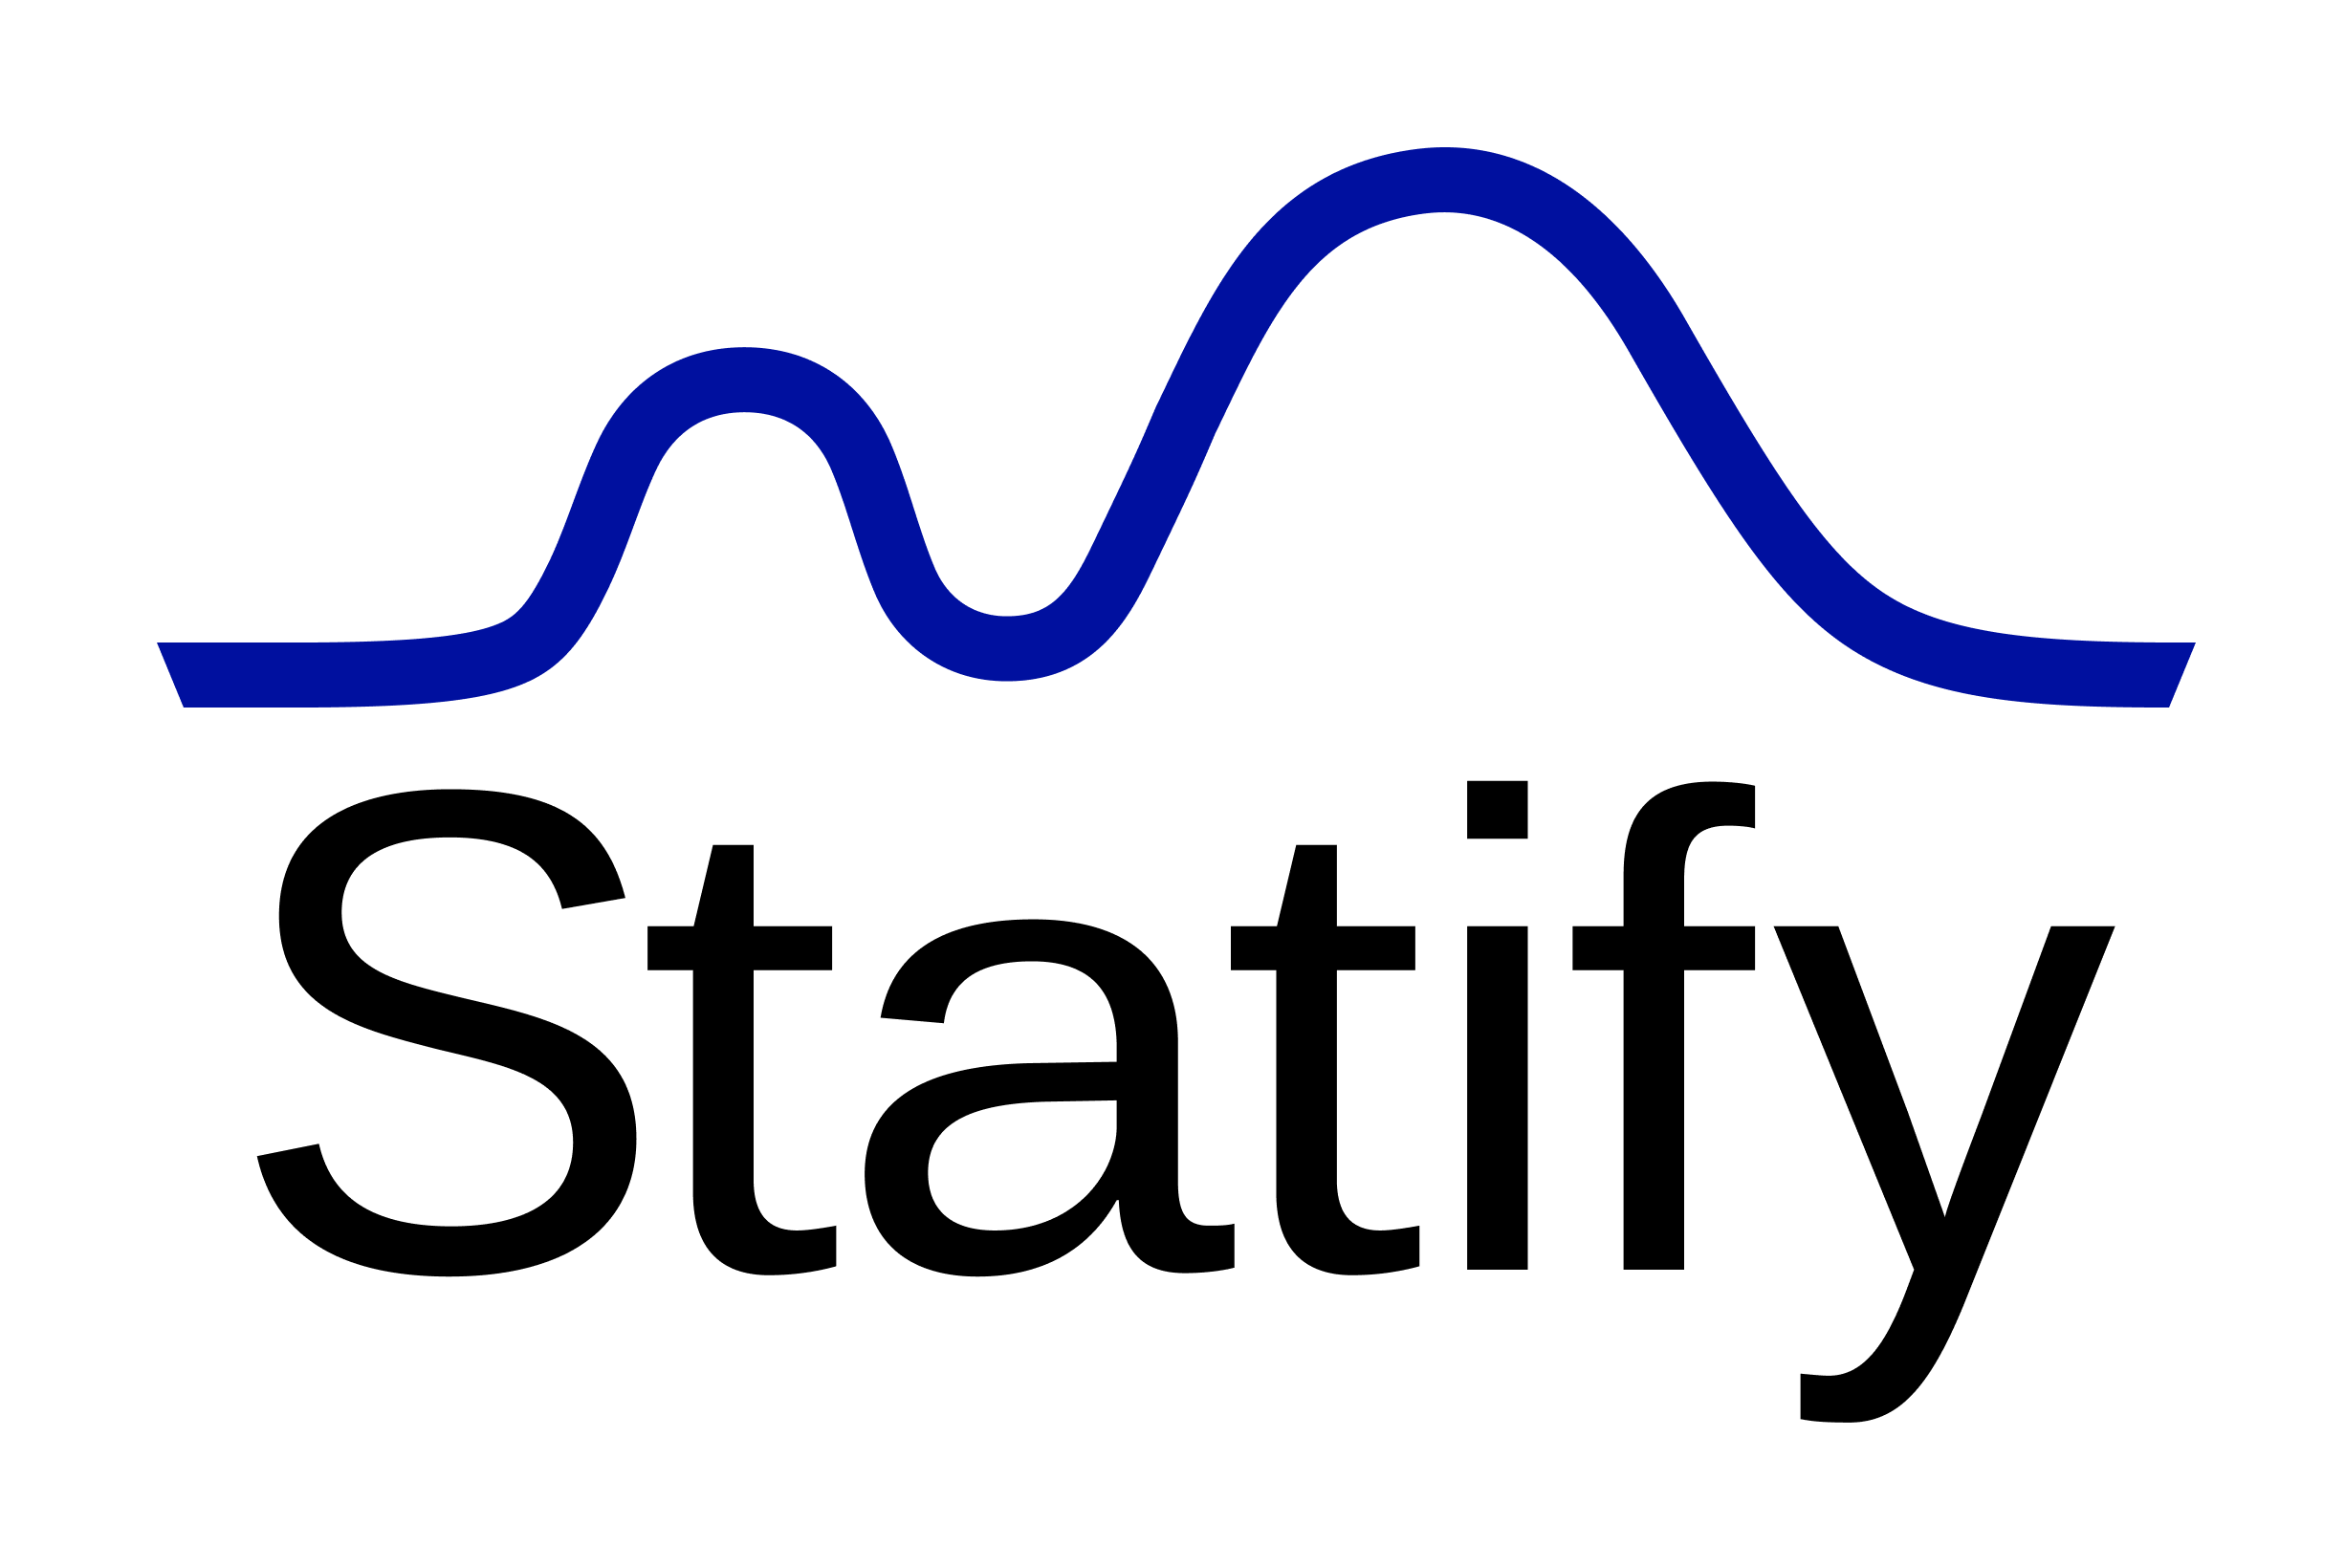
\includegraphics[width=0.3\textwidth]{figures_julyan/logo/statify.png}
}
\date{}
